\chapter{Корзины и мячи}
\label{ch:BucketsAndBalls}

Связанные данные по-прежнему в значительной степени неизвестны или неправильно поняты и недооценены. Часто людям это кажется слишком сложным. 
Поэтому я продолжаю искать новые способы сделать связанные данные более доступными. И с некоторым успехом. 
На сегодняшний момент на моих курсах более 60\% участников не имели опыта работы в области информационных технологий. Я надеюсь увеличить этот процент в будущем.

Самым сложным кажется написание SPARQL запросов. Специфика написана для ИТ-специалистов. Есть несколько отличных курсов и книг, но они также нацелены на людей с некоторым или большим опытом работы в сфере ИТ. Во всяком случае, это пугает остальных и удерживает SPARQL подальше от масс.

Я продолжаю учиться тому, что является сложным. Повторяющаяся и неожиданная проблема – это концепция переменной.

Что такое переменная в SPARQL? Просто заполнитель. Но как вы можете представить себе заполнитель? Это абстрактно. У нас нет способа постичь абстрактные вещи, если мы не ассоциируем их с чем-то физическим и конкретным. Трудно представить себе время, но как только мы рисуем его в пространстве, становится легче. Мы не можем представить мебель, но у нас нет проблем со стулом.

Другая проблема заключается в том, как выглядит запрос SPARQL. Хотя работа со SPARQL помогает понять, как работает граф знаний, запрос SPARQL на него не похож. Это как с символами в математике. <<5 не похоже на пять, в то время как ||||| равно пяти>>. Проблема со SPARQL аналогична:

\begin{quote}
Вы хотите запросить график знаний.\\
Вы хотите узнать что-то новое.\\
Но ваш запрос не похож на граф знаний.\\
Это похоже на линии струн.\\
\end{quote}

Итак, как вместе решить проблемы с захватом переменных и внешним видом SPARQL?

Я предлагаю представить каждый запрос SPARQL в виде графа связанных корзин и мячей.

Переменные являются заполнителями, но абстрактными. Нам нужен физический контейнер, чтобы наполнить его вещами. Нам нужны корзины. И вершины похожие на мячи. Итак, подумайте о выполнении запроса как о заполнении корзин мячами.

Тогда образец графа будет выглядеть так (рис. ~\ref{fig:graphPattern}):

\begin{marginfigure}[-1.5cm]
	{
		\setlength{\fboxsep}{0pt}%
		\setlength{\fboxrule}{1pt}%
		\fcolorbox{gray}{gray}{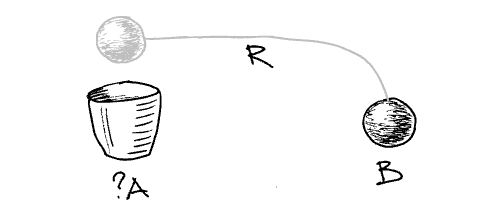
\includegraphics{./intro/bucketsAndBalls/graphPattern.PNG}}
	}
    \caption{Образец графа заполнения корзин мячами.}
	\label{fig:graphPattern}
\end{marginfigure}

Корзина \textbf{?A} должна быть заполнена теми мячами, которые имеют отношение \textbf{R} к мячу \textbf{B}.

Но это выглядит лучше, если мы сокращаем его так (рис. ~\ref{fig:graphPatternBucketsBalls}): 

\begin{marginfigure}[1.0cm]
	{
		\setlength{\fboxsep}{0pt}%
		\setlength{\fboxrule}{1pt}%
		\fcolorbox{gray}{gray}{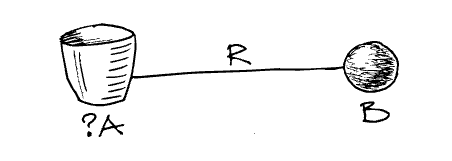
\includegraphics{./intro/bucketsAndBalls/graphPatternBucketsBalls.PNG}}
	}
    \caption{Шаблон графа в нотации <<Корзины и мячи>>.}
	\label{fig:graphPatternBucketsBalls}
\end{marginfigure}

Это шаблон графа в нотации <<Корзины и мячи>>. Направление отношения R не показано, но оно всегда слева направо.

Затем процесс написания и выполнения запроса SPARQL будет состоять из следующих этапов:
\begin{enumerate}
    \item Выберите свои корзины (в них вы собираетесь набирать нужные вам мячи).
    \item Составьте свои условия в виде графа корзин и мячей.
    \item Запустите свой запрос, чтобы заполнить ваши корзины мячами.
\end{enumerate}

Теперь давайте напишем запрос, чтобы получить всех глав правительств регионов, следуя этим шагам.

\begin{enumerate}
    \item Нам нужны две корзины, одна для регионов и одна для глав правительств.
    \item Корзина для региона должна быть привязано к мячу <<область России>> с отношением <<экземпляр>> и она должна быть связана с корзиной для <<главы правительства>>, которая, учитывая направление, следует рассматривать как <<имеет главу правительства>>. 
\end{enumerate}

\newpage
Давайте сделаем его более интересным и добавим еще одну корзину для изображений. Вот теперь запрос в нотации <<Корзины и мячи>>:

\begin{figure*}[h!]
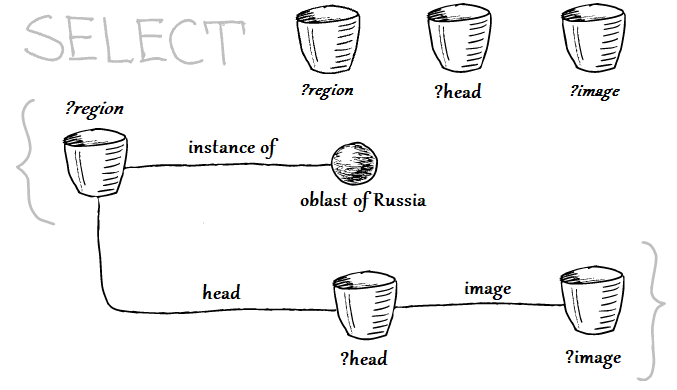
\includegraphics[width=0.6\linewidth]{./intro/bucketsAndBalls/select.PNG}
\end{figure*}

При выполнении запроса наши корзины должны выглядеть следующим образом (рис. ~\ref{fig:BucketsBallsQuery}): 

\begin{marginfigure}[1.0cm]
	{
		\setlength{\fboxsep}{0pt}%
		\setlength{\fboxrule}{1pt}%
		\fcolorbox{gray}{gray}{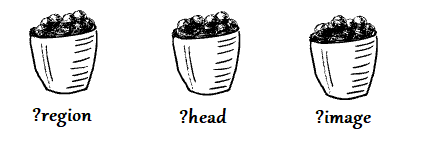
\includegraphics{./intro/bucketsAndBalls/query.PNG}}
	}
    \caption{Корзины при выполнении запроса.}
	\label{fig:BucketsBallsQuery}
\end{marginfigure}

Теперь давайте перейдем к Викиданным и напишем этот запрос там. Начните с выбора корзин для заполнения.

\begin{lstlisting}[ language=SPARQL ]
SELECT DISTINCT ?region ?head ?image
\end{lstlisting}

Далее нам нужно написать условия, которым должны соответствовать мячи для заполнения корзин. Все условия в SPARQL заключены в фигурные скобки {}.

Когда нам нужно определенное отношение или мяч, нам нужно использовать его идентификатор. Викиданные предоставляют хорошую услугу, которая записывает идентификатор для вас, как только вы выбираете отношение (свойство) или мяч (элемент) по его метке. Общая часть прямых отношений в графе знаний Викиданных сокращена с помощью wdt, а элементов (наших мячей) - с помощью wd.

Следуя нашему рисунку <<Корзины и мячи>>, мы начинаем писать условия, заполняя первую корзину ?region. Затем нам нужно написать первое отношение. Поскольку общей частью идентификаторов прямых отношений является wdt, мы пишем wdt:, а затем нажимаем Ctrl+пробел, чтобы запустить службу автозаполнения Викиданных (рис. ~\ref{fig:BucketsBallsProperty}).

\begin{marginfigure}[-2.5cm]
	{
		\setlength{\fboxsep}{0pt}%
		\setlength{\fboxrule}{1pt}%
		\fcolorbox{gray}{gray}{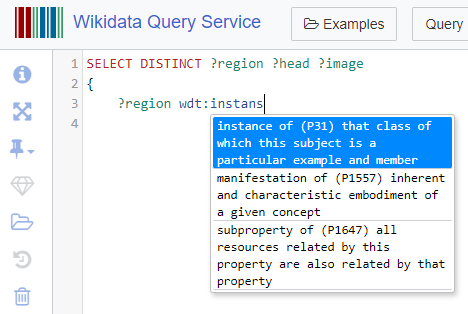
\includegraphics{./intro/bucketsAndBalls/property.PNG}}
	}
    \caption{Заполнение первой корзины.}
	\label{fig:BucketsBallsProperty}
\end{marginfigure}

После этого мы воспроизводем модель из рисунка <<Корзины и мячи>> в реальном запросе SPARQL.

Обычно при написании запроса SPARQL его приравнивают к виду таблицы с тремя столбцами: субъект, предикат, объект или на языке викиданных - элемент, свойство, значение.

(???) Но это укрепляет мышление в формате таблиц. Поэтому, возможно, было бы лучше, чтобы хотя бы ваши первые запросы напоминали граф. Ставя корзину как субъект нового графа (тройной шаблон) под той же корзиной, которая является объектом предыдущего тройного шаблона, делает его более похожим на граф с рисунка корзины и шары, который был представлен выше. Таким образом, наш запрос выглядит следующим образом:

\begin{lstlisting}[ language=SPARQL ]
SELECT DISTINCT ?region ?head ?image
{
    ?region wdt:P31 wd:Q835714; # oblast of Russia
    wdt:P6  ?head. # heads of government
    ?head  wdt:P18 ?image. # images of heads of government
}
\end{lstlisting}

Теперь посмотрите, как этот запрос выглядит в Викиданных, и запустите его. Затем нажмите на значок глаза слева и выберите, чтобы просмотреть результаты в виде сетки изображений.

\begin{figure*}[h!]
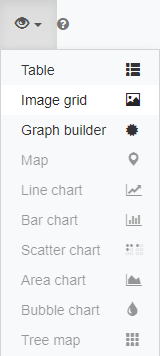
\includegraphics[width=0.5\linewidth]{./intro/bucketsAndBalls/imageGrid.PNG}
\end{figure*}

Это неплохо для первого результата, но теперь на каждом изображении мы видим только идентификационные данные людей и идентификационные данные их страны. Если мы нажмем на идентификатор, мы получим много информации об этом предмете. Но было бы лучше, если бы, помимо идентификаторов, мы могли видеть их метки в результате запроса. В основном это означает наклеивание этикеток на наши корзины. 

\begin{figure*}[h!]
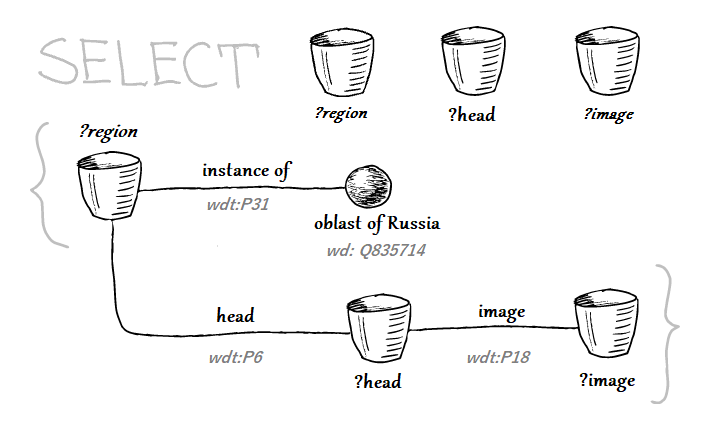
\includegraphics[width=0.6\linewidth]{./intro/bucketsAndBalls/selectID.PNG}
\end{figure*}

Label - это то, с чем связан каждый мяч, но Викиданные предоставляют его как услугу, поэтому вам не нужно об этом думать. Все, что вам нужно сделать, это: добавить слово “label” к переменным и вызвать службу меток. Последнее вы делаете, снова нажимая Ctrl+пробел в новой строке внутри {}, и когда вы начнете вводить “ярлык”, появится служба маркировки. По умолчанию вы получаете его с языком интерфейса и английским языком в качестве альтернативы, если метка недоступна на языке выбранного интерфейса Викиданных. Викиданные полны таких замечательных сервисов, и для окончательного запроса мы воспользуемся еще одним. Чтобы получить результат в сетке изображений по умолчанию, поместите где-нибудь в своем запросе следующий комментарий: \textcolor{blue}{\#defaultView:ImageGrid}

На самом деле вам не нужно все это писать. Когда вы начнете печатать, сервис автозаполнения предложит это.

Наш последний запрос выглядит так (листинг~\ref{lst:regionsOfHeads};): 

\begin{lstlisting}[ language=SPARQL, caption={\href{https://w.wiki/4ENR}{Список глав областей России}\protect\footnotemark}, label=lst:regionsOfHeads, ]
# List of regions of the Russian Federation and images of heads of government
#defaultView:ImageGrid
SELECT DISTINCT ?region ?regionLabel ?head ?headLabel ?image
{
  ?region wdt:P31 wd:Q835714; # ?region is Oblast of Russia
          wdt:P6  ?head.      #         has head of government
  ?head  wdt:P18 ?image.      # head has image
  SERVICE wikibase:label {bd:serviceParam wikibase:language "ru"} 
}
\end{lstlisting}
\footnotetext{Получено 44 области России и их глав правительства. Ссылка на SPARQL-запрос: \href{https://w.wiki/4ENR}{https://w.wiki/4ENR}}

Попробуйте это.

Я надеюсь, что представление о запросах SPARQL как связанных корзинах и мячах может быть полезным, по крайней мере, в начале. И, конечно, у каждой метафоры есть ограничения. Например, вы не можете поместить один и тот же мяч в две разных реальных корзины, но в эти виртуальные можете. Корзины и мячи могут быть полезной лестницей. Как только вы забрались наверх, вы можете пройти через это. (???)